% !TEX TS-program = pdflatex
% !TEX encoding = UTF-8 Unicode

%%% DOCUMENT DEFINITION
\documentclass[11pt, french]{article} % use larger type; default would be 10pt
\usepackage[utf8]{inputenc} % set input encoding (not needed with XeLaTeX)

%%% PAGE DIMENSIONS
\usepackage{geometry} % to change the page dimensions
\geometry{a4paper} % or letterpaper (US) or a5paper or....
\geometry{margin=1in} % for example, change the margins to 2 inches all round

%%% PACKAGES
\usepackage{graphicx} % support the \includegraphics command and options
\usepackage{booktabs} % for much better looking tables
\usepackage{array} % for better arrays (eg matrices) in maths
\usepackage{paralist} % very flexible & customisable lists (eg. enumerate/itemize, etc.)
\usepackage{verbatim} % adds environment for commenting out blocks of text & for better verbatim
\usepackage{subfig} % make it possible to include more than one captioned figure/table in a single float
\usepackage[frenchb]{babel}


%%% HEADERS & FOOTERS
%\usepackage{fancyhdr} % This should be set AFTER setting up the page geometry
%\pagestyle{fancy} % options: empty , plain , fancy

% Rapport projet pluridisciplinaire : etude thermique du pont en H
% : Xavier Galzin, Stanislas Bertrand, Romain Desille, Frédéric Meslin

\title{Projet pluridisciplinaire \\ Rapport Solution Analogique}
\author{Xavier GALZIN, Stanislas BERTRAND, Romain DESILLE, Frédéric MESLIN}
\date{19/03/2012}

\begin{document}
\maketitle

\pagebreak

\section*{Introduction}
Liste
\\- Rappel des objectifs
\\- liens avec l'étude automatique

\section{Capteur \& Conditionnement}
\subsection{Capteur à Effet Hall}
Liste
\\- Principe Générique
\\- Mise en Place sur la maquette
\\- Caractéristique principales des modules ( Alimentée, faible z, ... )
\\- Nécéssité de mesure différentielle
\subsection{Montage différentielle}
Liste
\\- Choix du montage + schema
\\- justification avantages / inconvengents
\\- Choix des AOPs ( Prix, Dispo, Package )
\\- Etude du montage
\\- Gain reglables
\\- Ajout d'un Offset 
\\- - Resultats des tests justifiant les valeurs ( cf section suivante )
\subsection{Consigne Analogique}
Liste
\\- Consigne numérique vers consigne analogique
\\- Retour : implantation analgoqie
\\- - Gain en précision (centrage sur l'offset)
\\- - Maximisation de la plage de conversion ( réajustement de l'offset )


\section{Correcteur Avance de phase}

Liste
\\- Choix du montage
\\- Choix dex couples R-C ( Cf Meca ) ( Choix des série E6, E12 et du type des condensateurs)
\\- Etude du gain du montage


\subsection{Données}

\noindent
Pour le schémas et les formules (que nous avons quand même vérifié) du correcteur, nous nous sommes servi d'un schémas trouvé sur internet (voir Bibliographie) :

\begin{center}
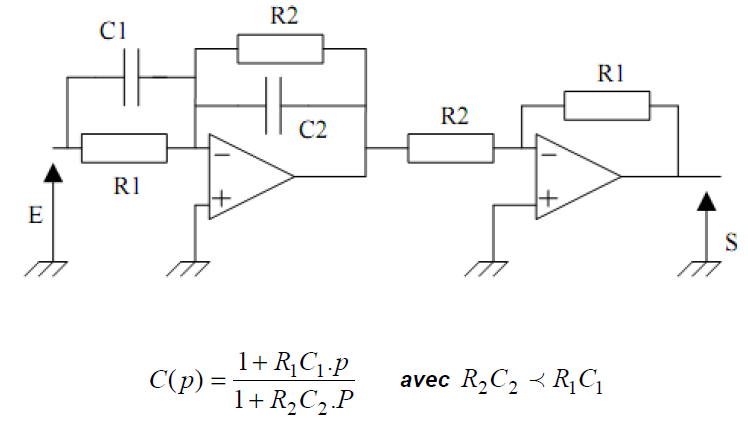
\includegraphics[width = 15cm]{SolutionAnalogique/Avph.png} 
\end{center}

\vspace{0.5cm}

Dans ce schémas, le produit $R_1*C_1$ correspond à la constante $ T_av$ définie dans le rapport d'automatique et le produit $R_2*C_2$ correspond à $0.1*T_av$.


Nous allons déterminer les valeurs de $R_1$, $R_2$, $C_1$ et $C_2$ dans deux configurations : poids du mobile à $0.0897 kg$ correspondant à un $T_av$ de 0.0313 et poids du mobile à $0.1414 kg$ correspondant à un $T_av$ de 0.0393.


Aussi, par le biais de MATLAB, nous avons pu obtenir la courbe théorique de notre correcteur par avance de phase :

\begin{center}
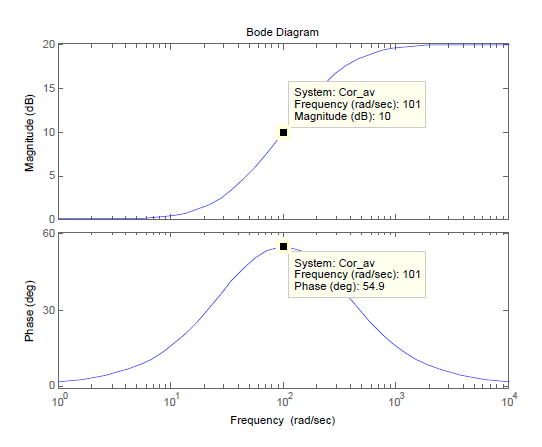
\includegraphics[width = 15cm]{SolutionAnalogique/aphmat.png} 
\end{center}

A noter que la fréquence donnée est en $rad.s^-1$, elle vaut environ 16Hz. 
\subsection{Détermination de valeurs des composants}

Pour des raisons de simplifications, nous prendrons les résistances $R_1$ et $R_2$ égales, le facteur 10 entre les constantes du numérateur et du dénominateur sera donc réalisé par un facteur 10 entre les valeurs des condensateurs. 



Pour le poids de $0.0897 kg$, en choisissant des composants avec des valeurs normalisées, on obtient $R=8.2 K\Omega$, $C_1=3.9 \mu F$ et $C_2=390 nF$. 



On fera plutôt varier les résistances que les condensateurs pour s'adapter au changement de poids. On conserve donc les mêmes valeurs de condensateurs. On trouve alors $R=10.076 K\Omega$. 



Il sera donc possible de prendre des potentiomètres pour ajuster les constantes, corrigeant ainsi les écards possibles des valeurs de condensateurs. 


\subsection{Validation par simulation PSpice}

On simule le correcteur à avance de phase par le schémas suivant : 

\begin{center}
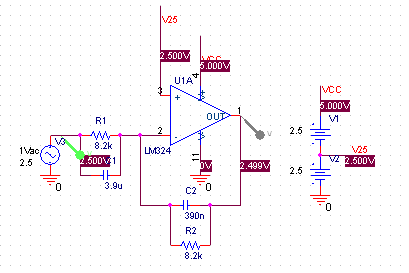
\includegraphics[width = 15cm]{SolutionAnalogique/schAvph.png} 
\end{center}

On obtient le résultat de simulation suivant : 

\begin{center}
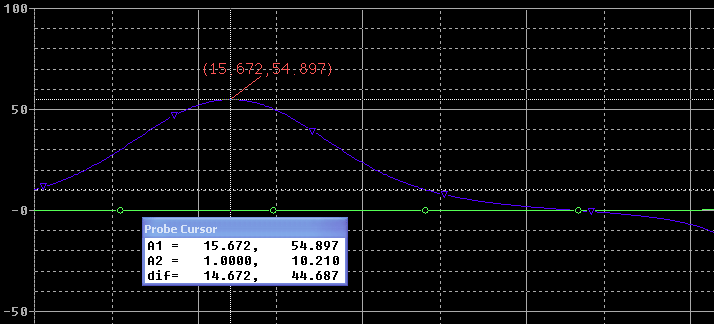
\includegraphics[width = 15cm]{SolutionAnalogique/simuAvph.png} 
\end{center}

Comme on peut le voir en comparant par rapport au résultat donné par MATLAB, le schéma répond comme on le souhaitait. 

\vspace{0.5cm}
\subsection{Conclusion}

\noindent
Nous avons donc validé notre choix de montage de correcteur et nous avons déterminer des valeurs admissibles de composants analogiques grâce à cette étude. Il faudra cependant être attentif quant au choix des condensateurs vis-à-vis de leur fréquence de fonctionnement.  

\subsection{Bibliographie}

- Cours de GEE, A. Meghebbar :
\newline \textit{\underline{fsi.univ-tlemcen.dz/cours/Support-Cours-Commande-Analogique-Master-Electrotechnique10.pdf}}


\section{Conversion \& Comunication}
\subsection{Choix du microcontrolleur}
Liste
\\- Tension d'alimentation
\\- Frequence de travail
\\- module de conversion
\\- Disponibilité des outils de dev
\\- instructions evoluées MUL \& DIV pour le correcteur numérique

\subsection{Conversion A/D - PWM}
Liste
\\- Utilisation des modules
\\- Programme + Explications

\subsection{Communication serie/USB}
Liste
\\- Ajout d'un driver USB/Série
\\ Programme le cas échéant

\section{Control de puissance}
Liste
\\- choix du pont complet ( Justification )
\\-  - Attraction | Répulsion de la bobine
\\-  - Asservissement à l'équilibre ?
\\- Choix du composant
\\- Réalisation PCB
\\-  - Problème thermique
\\-  - Problème de boitier
\\- Utilisation du four à réfusion

\subsection{Données}

\noindent
D'après la Datasheet du A4950 :

\vspace{0.5cm}

\noindent
$ 
R_{TH} = 62 \char123C/W  \\
T_{JUNC\_MAX} = 160 \char123C  \\
T_{AMB} = 25\char123C  \\
R_{DSON} = 1.3 \Omega  \\
$



\noindent
A noter que cette valeur de $R_{TH}$ est donnée dans le cas l'on a aurait des plages de cuivres d'environ 2cm par 2cm de chaque côté du composant. De plus, la valeur de $R_{DSON}$ est une valeur pire cas.

\subsection{Equations}

\noindent
L'équation de la température de la jonction est donnée par :

\vspace{0.5cm}

\noindent
$
T_{JUNC} = R_{TH} * P_{DIS} + T_{AMB}
$

\vspace{0.5cm}

\noindent
P étant la puissance \textbf{dissipée} dans le composant que l'on calculera par la formule :

\vspace{0.5cm}

\noindent
$
P_{DIS} = R_{DSON} * I\up{2} = 1.3 * 1.28\up{2} = 5.2 W
$

\vspace{0.5cm}

\noindent
Finalement, on obtient :

\vspace{0.5cm}

\noindent
$
T_{JUNC} = 62 * 5.2 + 25 = 157.06 \char123C
$

\subsection{Conclusion}

\noindent
Le résultat trouvé est très proche de la valeur limite du composant. Cependant, nous avons pris des paramètres extrèmes qui ne seront normalent pas atteint. De plus, nous comptons augmenter la surface de cuivre qui assurera la dissipation afin d'obtenir une marge plus grande par rapport à ce résultat.

\section{Résultats - Evolution}
Liste
\\- Monitoring du fonctionnement
\\- Résulatat expérience
\\- Ouverture vers correcteur numérique

\end{document}
